

\subsubsection{Dipole Moments}
\label{cl:dipole-moments}

%%%%%%%%%%%%%%%%%%%%%%%%%%%%%%%%%%%
% For all our labels we use :cl: (cl for charged leptons), like
% eq:cl:mueg
% That way we will not have problems when combining it

%%%%%%%%%%%%%%%%%%%%%%%%%%%%%%%%%%%%%%%%%%%%%%%%%%%%%%%%%%%
%%%%%%%%%%%%%%%%%%%%%%%%%%%%%%%%%%%%%%%%%%%%%%%%%%%%%%%%%%%
%%%%%%%%%%%%%%%%%%%%%%%%%%%%%%%%%%%%%%%%%%%%%%%%%%%%%%%%%%%
%%%%%%%%%%%%%%%%%%%%%%%%%%%%%%%%%%%%%%%%%%%%%%%%%%%%%%%%%%%


The muon provides a unique opportunity to explore the properties of a
second-generation particle  with great precision. Several muon properties make
these measurements possible.  It has a long
lifetime of $\simeq 2.2~\mu$s,  it is produced in the weak decay
$\pi^- \rightarrow \mu^- \bar \nu_\mu$ providing copious numbers of
polarized muons, and the weak decay
$\mu^- \rightarrow e^- \nu_\mu \bar \nu_e $ is self-analyzing providing information on the muon spin direction at the time of decay.

In his famous paper on the relativistic theory of the electron,
Dirac\cite{Dirac28} obtained the correct magnetic moment for the
electron, and he also mentioned the possibility of an electric
 dipole moment, which like the magnetic dipole moment,
would be directed along the electron spin direction.
  The magnetic dipole (MDM) and electric dipole (EDM)
moments are given by
\begin{equation}
\vec \mu = g \left( \frac{Qe}{ 2m}\right) \vec s\, , \qquad
 \vec d = \eta  \left(\frac {Qe  }{ 2
     mc}\right)
\vec s \, ,
\label{eq:MDM-EDMdef}
\end{equation}
where  $Q =  \pm 1$ and $e>0$. Dirac theory predicts $g \equiv 2$,
but radiative corrections dominated by the
lowest-order (mass-independent) Schwinger contribution $a_{e,\mu,\tau} =
 \alpha/(2\pi)$~\cite{Schwinger48} make it necessary to
write the magnetic moment as
\begin{equation}
\mu = \left(1 + a\right)\frac{Qe \hbar }{ 2m}\quad {\rm with} \quad
a = \frac{{g - 2} }{ 2}.
\label{eq:muon-MDM}
\end{equation}

The muon played an important role in our discovery of the generation
structure of the Standard Model (SM) when
 experiments at the Nevis
cyclotron
showed  that $g_\mu$ was consistent with 2~\cite{Garwin57}.
Subsequent experiments at Nevis and CERN showed  that
$a_\mu \simeq \alpha/(2\pi)$~\cite{Garwin60,Charpak61},
implying that in a magnetic field, the muon
behaves like a heavy electron.
The SM value of the muon anomaly is now known
to better than half a part per million (ppm), and has
been measured to a similar precision~\cite{Bennett06}.

The quantity $\eta$ in Eq.~\ref{eq:MDM-EDMdef}
 is analogous to the $g$-value for the magnetic dipole
moment. An EDM violates both {\sl P} and {\sl T}
symmetries~\cite{Purcell50,Landau57,Ramsey58}, and since $C$ is conserved,  ${ C\!P}$ is violated as well.  Thus
searches for EDMs provide an important tool in our quest to
find non-Standard Model ${ C\!P}$ violation.

The measured value of the muon anomalous magnetic moment is in apparent
disagreement with the expected value based on the
SM.  The BNL E821 experiment finds~\cite{hep-ex/0602035}
\begin{equation} \hspace*{-23pt}
    a_\mu(\textrm{Expt}) = 116\,592\,089(54)(33)\times10^{-11},
    \label{eq:e821}
\end{equation}
where $a_\mu=(g-2)/2$ is the muon anomaly, and the uncertainties are
statistical and systematic, respectively.  This can be compared with
the SM prediction~\cite{arXiv:1010.4180,931465}
\begin{equation}
    a_\mu(\textrm{SM})   = 116\,591\,802(42)(26)(02)\times10^{-11},
    \label{eq:SM}
\end{equation}
where the uncertainties are from the $\mathrm{O}(\alpha^2)$ hadronic vacuum
polarization (HVP) contribution, $\mathrm{O}(\alpha^3)$ hadronic
contributions (including hadronic light-by-light (HLbL) scattering),
and all others (pure QED, including a 5-loop
estimate~\cite{arXiv:1110.2826}, and electroweak, including
2-loops~\cite{hep-ph/0212229}). The hadronic contributions dominate
the uncertainty in $a_\mu(\rm SM)$.  The discrepancy between the
measurement and the SM stands at
\begin{equation}
\Delta a_\mu=287(80)\times 10^{-11}
\end{equation}
(3.6 standard deviations ($\sigma$)), when based on the $e^+e^-\to\rm
hadrons$ analysis for the HVP
contribution~\cite{arXiv:1010.4180}. When the HVP analysis is
complemented by $\tau\to\rm hadrons$, the discrepancy is reduced to
2.4$\sigma$~\cite{arXiv:1010.4180}. However, a recent re-analysis,
employing effective field theory techniques, of the $\tau$
data~\cite{arXiv:1101.2872} shows virtual agreement with the
$e^+e^-$-based analysis, which would solidify the current discrepancy
at the 3.6$\sigma$ level. $\Delta a_\mu$ is large, roughly two times
the EW contribution~\cite{hep-ph/0212229}, indicating potentially
large new physics contributions.



%%% BSM


The anomalous magnetic moment of the muon is sensitive to
contributions from a wide range of physics beyond the standard
model. It  will continue to place stringent restrictions on all of
the models, both present and yet to be written down. If  
physics beyond the standard model is discovered at the LHC 
or other experiments,
$a_\mu$  will constitute an indispensable tool to discriminate
between very different types of new physics, especially since it is
highly sensitive to parameters which are difficult to measure at the
LHC. If no new phenomena are found elsewhere, then it represents one of the few ways
to probe physics beyond the standard model. In either case, it will play an
essential and complementary role in the quest to understand physics
beyond the standard model at the TeV scale. 

The muon magnetic moment has a special role because it is
sensitive to a large class of models related and unrelated to electroweak symmetry breaking and
because it combines several properties in a unique way: it is a
flavor- and CP-conserving, chirality-flipping and loop-induced 
quantity. In contrast, many high-energy collider observables at the
LHC and a future linear collider are chirality-conserving, and many
other low-energy precision observables are CP- or
flavor-violating. These unique properties might be the reason why the
muon $(g-2)$ is the only among the mentioned observables which shows a 
significant deviation between the experimental value and the SM
prediction.  Furthermore, while $g-2$ is sensitive
to leptonic couplings, 
$b$- or $K$-physics more naturally probe the hadronic couplings of new
physics. If charged lepton-flavor violation exists, observables such
as $\mu\to e$ conversion can only determine a combination of the
strength of lepton-flavor violation and the mass scale of new
physics. In that case, $g-2$ can help to disentangle the nature of the
new physics. 


((( I would like to reduce this entire thing below to one table.  BCKC)))))

Unravelling the existence and the properties of such new physics
requires experimental information complementary to the LHC.
The muon $(g-2)$, together
with searches for charged lepton flavor violation, electric dipole
moments, and rare decays, belongs to a class of complementary
low-energy experiments.

In fact, 
The role of $g-2$ as a discriminator between very different standard
model extensions is well illustrated by a relation stressed by
Czarnecki and Marciano~\cite{czmar}. It holds in a wide range of
models as a result of the chirality-flipping nature of both  $g-2$ and
the muon mass: If a new
physics model with a mass scale $\Lambda$
contributes to the muon mass $\delta m_\mu(\mbox{N.P.})$, it also
contributes to $a_\mu$, and the two contributions are related as
\begin{equation}
\label{CzMbound} a_\mu(\mbox{N.P.})={\cal O}(1)\times
\left(\frac{m_\mu}{\Lambda}\right)^2 \times \left(\frac{\delta
m_\mu(\mbox{N.P.})}{m_\mu}\right). 
\end{equation}


The ratio $C(\mbox{N.P.})\equiv\delta m_\mu(\mbox{N.P.})/{m_\mu}$
cannot be larger than unity unless there is fine-tuning in the muon
mass. Hence a first consequence of this relation is that new physics
can explain the currently observed deviation (\ref{eq:Delta}) only if
$\Lambda$ is at the few-TeV scale or smaller.

In many models, the ratio $C$ arises from one- or even two-loop
diagrams, and is then suppressed by factors like  $\alpha/4\pi$ or
$(\alpha/4\pi)^2$. Hence, even for a given $\Lambda$, the
contributions to $a_\mu$ are highly model dependent.

It is instructive to classify new physics models as follows:
\begin{itemize}
\item Models with $C(\mbox{N.P.})\simeq1$: Such models are of interest
  since the muon
  mass is essentially generated by radiative effects  at some
scale $\Lambda$.
A variety of such models  have been discussed in~\cite{czmar}, including
extended technicolor or generic models with naturally vanishing bare
muon mass. For examples of radiative muon mass generation within
supersymmetry, see e.g.\ 
\cite{Borzumati:1999sp,Crivellin:2010ty}.  In these models the
new physics contribution to $a_\mu$ can be very large, 
\begin{equation} 
a_{\mu}
(\Lambda) \simeq {m^2_{\mu} \over \Lambda^2}\simeq
1100\times10^{-11}\left(\frac{1\mbox{ TeV}}{\Lambda}\right)^2. 
\end{equation}
and the difference Eq.~(\ref{eq:Delta}) can  be used to place a lower
limit on the new physics mass scale, which is in the few TeV
range~\cite{elp,Crivellin:2010ty}.
\item Models with $C(\mbox{N.P.})={\cal O}(\alpha/4\pi)$:
Such a loop suppression happens in many models with new weakly
interacting particles like $Z'$ or $W'$, little Higgs or certain extra
dimension models.  As examples, the contributions to $a_\mu$ in a
model with $\delta=1$ (or
2) universal extra dimensions (UED)~\cite{AppelqDob} and the Littlest Higgs
model with T-parity (LHT)~\cite{Blanke:2007db} are given by
% , other measurements already imply a
%lower bound of 300 (or 500) GeV on the masses of the extra states,
%and the one-loop contributions to  a_\mu\ are correspondingly small,
%\begin{equation}
 %a_\mu(\mbox{UED})&\simeq&-5.8\times10^{-11}(1+1.2\delta)S_{\rm
 % KK},\\
% a_\mu(\mbox{LHT})&<& 12\times10^{-11}
%\end{equation}
 with $|S_{\rm KK}| _{\sim}^{<}1$~\cite{AppelqDob}.
A difference as large as
Eq.~(\ref{eq:Delta}) is very hard to accommodate unless the mass scale
is very small, of the order of $M_Z$, which however is often excluded
e.g.\ by LEP measurements.
So typically these models predict very small contributions to $a_\mu$
and will be disfavored if the current deviation will be confirmed by
the new $a_\mu$ measurement.

Exceptions are provided by models where new particles
interact with muons but are otherwise hidden from searches. An example
is the model with a new gauge boson associated to a gauged lepton
number $L_\mu-L_\tau$ \cite{LmuLtau}, where a gauge boson mass of
${\cal O}(100\mbox{ GeV})$ and large $a_\mu$ are viable.
\item Models with intermediate values for $C(\mbox{N.P.})$ and mass
  scales around the weak scale: In such
  models, contributions to $a_\mu$ could be as large as
  Eq.~(\ref{eq:Delta}) or even larger, or smaller, depending on the
  details of the model. This implies that a more precise
  $a_\mu$-measurement will have significant impact on such models and
  can even be used to measure model parameters. Supersymmetric (SUSY) models
  are the best known examples, so muon $g-2$ would have substantial
  sensitivity to
 SUSY particles.
Compared to generic perturbative models,
supersymmetry provides an enhancement to $C(\mbox{SUSY})={\cal
  O}(\tan\beta\times\alpha/4\pi)$
and to $ a_\mu(\mbox{SUSY})$ by a factor $\tan\beta$ (the ratio of
the vacuum expectation values of the two Higgs fields). Typical SUSY
diagrams for the magnetic dipole moment, the electric dipole moment,
and the lepton-number violating conversion process $\mu \rightarrow
e$ in the field of a nucleus are shown pictorially in
Fig.~\ref{fg:susy}. The shown diagrams contain the SUSY partners of
the muon, electron and the SM U(1)$_Y$ gauge boson, $\tilde{\mu}$,
$\tilde{e}$, $\tilde{B}$. The full SUSY contributions involve also the
SUSY partners to the neutrinos and all SM gauge and Higgs bosons. In a
model with SUSY masses equal to $\Lambda$ 
the SUSY contribution to $a_{\mu}$ is given
by~\cite{czmar} \begin{equation} \label{amususy}
%&\simeq& {\alpha(M_Z) \over 8 \pi \sin^2 \theta_W} {m^2_{\mu} \over \tilde
%    m^2}
%\tan \beta \left( 1 - {4\alpha \over \pi}\ln {\tilde m \over m_{\mu}}\right)
%  \\
 a_{\mu}({\rm SUSY})\, \simeq \,{\rm sgn}\, (\mu) \ 130 \times 10^{-11}\ \tan \beta\
\left({100\ {\rm GeV}  \over \Lambda}\right)^2
%\\
% &\simeq& \ {1.31}\ \  {\rm ppm }  \ \ \  \tan \beta\
%  \left({100\ {\rm GeV} \over \tilde m}\right)^2 \\
\end{equation}
which indicates the dependence on $\tan \beta$,
and the SUSY mass scale,  as well as the sign of the
SUSY $\mu$-parameter. The formula still approximately applies even if
only the smuon and chargino masses are of the order $\Lambda$
but e.g.\ squarks and gluinos are much heavier. However the SUSY
contributions to $a_\mu$ depend strongly on the details of mass
splittings between the weakly interacting SUSY particles.
Thus muon $g-2$ is sensitive to  SUSY models with SUSY masses
in the few hundred GeV range, and it will help to measure SUSY
parameters. 

There are also non-supersymmetric models with similar
enhancements. For instance, lepton flavor mixing can help. An example
is provided in Ref.\ \cite{BarShalom:2011bb} by a model with two Higgs
doublets and four generations, which can accommodate large
$\Delta a_\mu$ without violating constraints on lepton flavor
violation. In variants of Randall-Sundrum models
\cite{Davoudiasl:2000my,Park:2001uc,Kim:2001rc} and large
extra dimension models \cite{Graesser:1999yg}, large
contributions to $a_\mu$ might be possible from exchange of
Kaluza-Klein gravitons, but the theoretical evaluation
is difficult because of cutoff dependences. A recent evaluation of the
non-graviton contributions in Randall-Sundrum models, however,
obtained a very small result \cite{Beneke:2012ie}. 



Further examples
include scenarios of unparticle physics
\cite{Cheung:2007zza,Conley:2008jg} (here a more precise
$a_\mu$-measurement would constrain the unparticle scale dimension and
effective couplings), generic models with a hidden sector at the weak
scale \cite{McKeen:2009ny} or a model with the discrete flavor 
symmetry group $T'$ and Higgs triplets \cite{Ho:2010yp} (here
a more precise $a_\mu$-measurement would constrain hidden sector/Higgs
triplet masses and couplings), or the model proposed in
Ref.\ \cite{Hambye:2006zn}, which implements the idea that neutrino
masses, leptogenesis and the deviation in $a_\mu$ all originate from
dark matter particles. In the latter model, new leptons and scalar
particles are predicted, and $a_\mu$ provides significant constraints
on the masses and Yukawa couplings of the new particles.
\end{itemize}

%
The following types of new physics scenarios are quite different from
the ones above:
\begin{itemize}
\item Models with extended Higgs sector but without the
  $\tan\beta$-enhancement of SUSY models. Among these models are the
  usual two-Higgs-doublet models. The one-loop contribution
  of the extra Higgs states to $a_\mu$ is suppressed by two additional powers of
  the muon Yukawa coupling, corresponding to $a_\mu(\mbox{N.P.})\propto
  m_\mu^4/\Lambda^4$ at the one-loop level. Two-loop effects from
  Barr-Zee diagrams can be larger \cite{Krawczyk:2002df}, but typically the
  contributions to   $a_\mu$ are negligible in these models.
\item Models with additional light particles with masses below the
  GeV-scale, generically called dark sector models: Examples are
  provided by the  models of   Refs.\
  \cite{Pospelov:2008zw,Davoudiasl:2012qa}, where additional light
  neutral gauge bosons can affect electromagnetic interactions. Such
  models are intriguing since 
  they completely decouple $g-2$ from the physics of EWSB, and since
  they are hidden from collider searches at LEP or LHC (see however
  Refs.\ \cite{Essig:2009nc,Davoudiasl:2012ig} for studies of possible
  effects at dedicated low-energy colliders and in Higgs decays at the
  LHC). They can lead to
  contributions to $a_\mu$ which are of the same order as the deviation
  in Eq.~(\ref{eq:Delta}). Hence the new $g-2$ measurement will provide
  an important test of such models.
\end{itemize}
To summarize:
many well-motivated models can accommodate larger contributions to
$a_\mu$ --- if any of these are realized $g-2$ can be used to constrain
model parameters; many well-motivated new physics models
give tiny contributions to $a_\mu$ and would be disfavored if the
more precise $g-2$ measurement confirms the current deviation. There are also examples of models which lead to
similar LHC signatures but which can be distinguished using $g-2$.



%%%%%%%%%%%%%%%%% DS references %%%%%%%%%%%%%





\subsection{Muon $g-2$: Experiment}\label{sec:cl:g-2exp}


Measurements of the magnetic and electric dipole moments make use of the
torque on a dipole in an external field, $\vec \tau = \vec\mu \times
\vec B + \vec d \times \vec E$. All muon MDM experiments except the original
Nevis ones used polarized muons in flight, and
 measured the rate at which the spin turns relative to the momentum,
$\vec \omega_a =\vec \omega_S - \vec \omega_C$, when a
 beam of polarized muons is injected into a magnetic field.
The resulting frequency, assuming that $\vec \beta \cdot \vec B = 0$,
 is given
by~\cite{Thomas26,Bargmann59}
\begin{equation}
\vec{\omega}_{a\eta}= \vec \omega_a + \vec \omega_\eta = -
 \frac {Qe}  {m}
\left[
a \vec{B}
+ \left( a - \left(  \frac {m} {p} \right)^2  \right)
 \frac {\vec{\beta} \times \vec{E}} {c} \right] -  \eta \frac {Qe}{2m}
 \left[ \frac {\vec{E}} {c}  +  \vec{\beta} \times \vec{B} \right] .
 \label{eq:omegaa-edm1}
\end{equation}
Important features of this equation are the motional magnetic and
electric fields:
$\vec \beta \times \vec E$ and $\vec \beta \times \vec B$.


The E821 Collaboration working at the
Brookhaven AGS used an electric quadrupole field
to provide vertical focusing in the storage ring, and shimmed the magnetic
field to 1 ppm uniformity on average.  The storage ring was operated
 at the `` $g-2$'' momentum, $p_{ g-2} = 3.094$~GeV/c,
($\gamma_{ g-2}= 29.3$),
so that $a_\mu = (m/p)^2$ and the electric field did not
contribute to $\omega_a$.
They obtained\cite{Bennett06}
\begin{equation}
  a_\mu^{(\mathrm{E821})} = 116\,592\,089(63) \times
  10^{-11}~~\mbox{(0.54\,ppm)}
\end{equation}
 The final uncertainty of
0.54~ppm consists of a 0.46~ppm statistical component and a 0.28~ppm
systematic
component.  

The present limit on the EDM also comes from E821~\cite{Bennett08-edm}
\begin{equation}
d_\mu = (0.1 \pm 0.9) \times 10^{-19} e  \cdot {\rm cm}; \
 \vert d_\mu \vert < 1.9 \times 10^{-19}  e  \cdot {\rm cm}\ (95\%\ {\rm C.L.})\, ,
\label{muedm-result}
\end{equation}
so the EDM contribution to the precession is very small.  In the muon $g-2$
experiments, the motional electric field dominates the $\omega_\eta$ term,
which means that $\vec \omega_a$ and $\vec \omega_\eta$ are orthogonal.
The presence of an EDM in the  $g-2$ momentum experiments has two effects:
the measured frequency is the quadrature sum of the two frequencies,
 $\omega = \sqrt{\omega_a^2 + \omega_\eta^2}$, and the EDM causes a tipping of
 the plane of precession, by an angle
 $\delta = \tan ^{-1}[ \eta \beta/(2a_\mu)]$. This tipping results in
 in an up-down oscillation of the decay
 positrons relative to the midplane of the storage ring with frequency
$\omega_a$ {\it out of phase by} $\pi/2$ with the $a_\mu$ precession.





\subsubsection{ Future $g-2$ Experiments}

The E989 collaboration
at Fermilab will move the E821 muon storage ring to Fermilab, and
will use the  $g-2$ momentum technique to measure $a_{\mu^+}$.
 New detectors and electronics, and a
beam handling scheme that increases the stored muon rate per hour
 by a factor of 6
over E821 will be implemented.  The goal is at least 21 times the
statistics of E821, and a factor of four overall uncertainty reduction, with
equal systematic and statistical uncertainties of $\pm 0.1$ ppm.

The scope of Project X includes 50-200kW of beam power at 8 GeV,
about three to fifteen times the beam power of E989.  This large step in beam
power could be used to measure $g-2$ for negative muons,
and provide muon beams with lower emittance thereby reducing
experimental systematics. 

Given the high impact of the E821 result and the 
crucial role the value of $g-2$ plays in interpreting energy frontier results, 
it is imperative to have a second measurement with at least equal 
precision but with a complementary approach to the measurement. 
An alternate approach planned for J-PARC~\cite{JPARC-Lg2} uses a much lower muon
energy, and does not use the  $g-2$ momentum technique. A surface muon beam
produced by  the low energy Booster is brought to rest in an aerogel
target, where muonium (the $\mu^+ e^-$ atom) is formed.  The muonium
is ionized by a powerful laser which produces a very slow muon beam with
extremely small emittance. This low emittance beam is then accelerated by a
linac to 300 MeV, and injected into a  $\sim 1$~m diameter
solenoidal magnet with point to point
uniformity of $\pm 1$ ppm, approximately 100 times better than at the Brookhaven experiment.  
The average uniformity is expected to be known to better then 0.1 ppm.  The decays are detected 
by a full volume tracker consisting of an array of silicon
detectors.  This provides time, energy, and decay angle information for every positron, maximizing
 the sensitivity to separate the  $g-2$ and EDM precession frequencies.  The expected   $g-2$ sensitivity 
 is comparable to the
 Fermilab experiment but will have very different systematic uncertainties and the combined results 
 from the two experiments should bring the precision to below the 100 ppb level.


\subsection{Muon $g-2$: Expected Improvements in the predicted value}\label{sec:cl:g-2exp}

((((( This can be shortened, updated, and add a table that has the expected improvements )))))


The QED and e;ectroweak contributions to $g-2$ can be calculated to from first principles and
and are regarded as robust.  The two dominant QCD contributions are hadronic vacuum polarization(HPV) and hadronic light-by-light contribution (HLBL) 
The HVP contribution to $a_\mu$ can be determined from the
cross-section for $e^+e^-\to\rm hadrons$ (and over a certain energy
range, by $\tau\to\rm hadrons$) and a dispersion relation. It can also
be computed from purely first principles using lattice QCD to
calculate the HVP directly~\cite{hep-lat/0212018}. The two methods are
complementary and can be used to check each other. The current best
uncertainty comes from the first method,
\begin{equation}
a_\mu(\rm HVP)=(692.3\pm4.2)\times 10^{-10},
\end{equation}
or about 0.61\%~\cite{arXiv:1010.4180} when only $e^+e^-$ data are used. 
If $\tau$ data are included, $a_\mu=701.5\pm4.7\times 10^{-10}$, or 0.67\% 
(but see~\cite{arXiv:1101.2872} for the analysis that brings the $\tau$ 
into good agreement with $e^+e^-$). In the next 3-5 years the uncertainty on 
$a_\mu(\rm HVP)$ is expected to drop by roughly a factor of 2, relying 
on new results from {\babar}, Belle, BES, and VEPP2000.
The lattice calculations presently have an uncertainty of 
about 5\%~\cite{hep-lat/0608011, arXiv:1103.4818, Boyle:2011hu,  DellaMorte:2011aa}, which is 
expected to decrease to 1-2\% in the next 3-5 years~\cite{USQCD}. At the 
one-percent level contributions from the charm and so-called disconnected 
diagrams (right panel, Fig.~\ref{fig:hvp}) enter. Both are currently under investigation.
%
\begin{figure}[bp]
    \centering
    %\vspace*{-3em}
    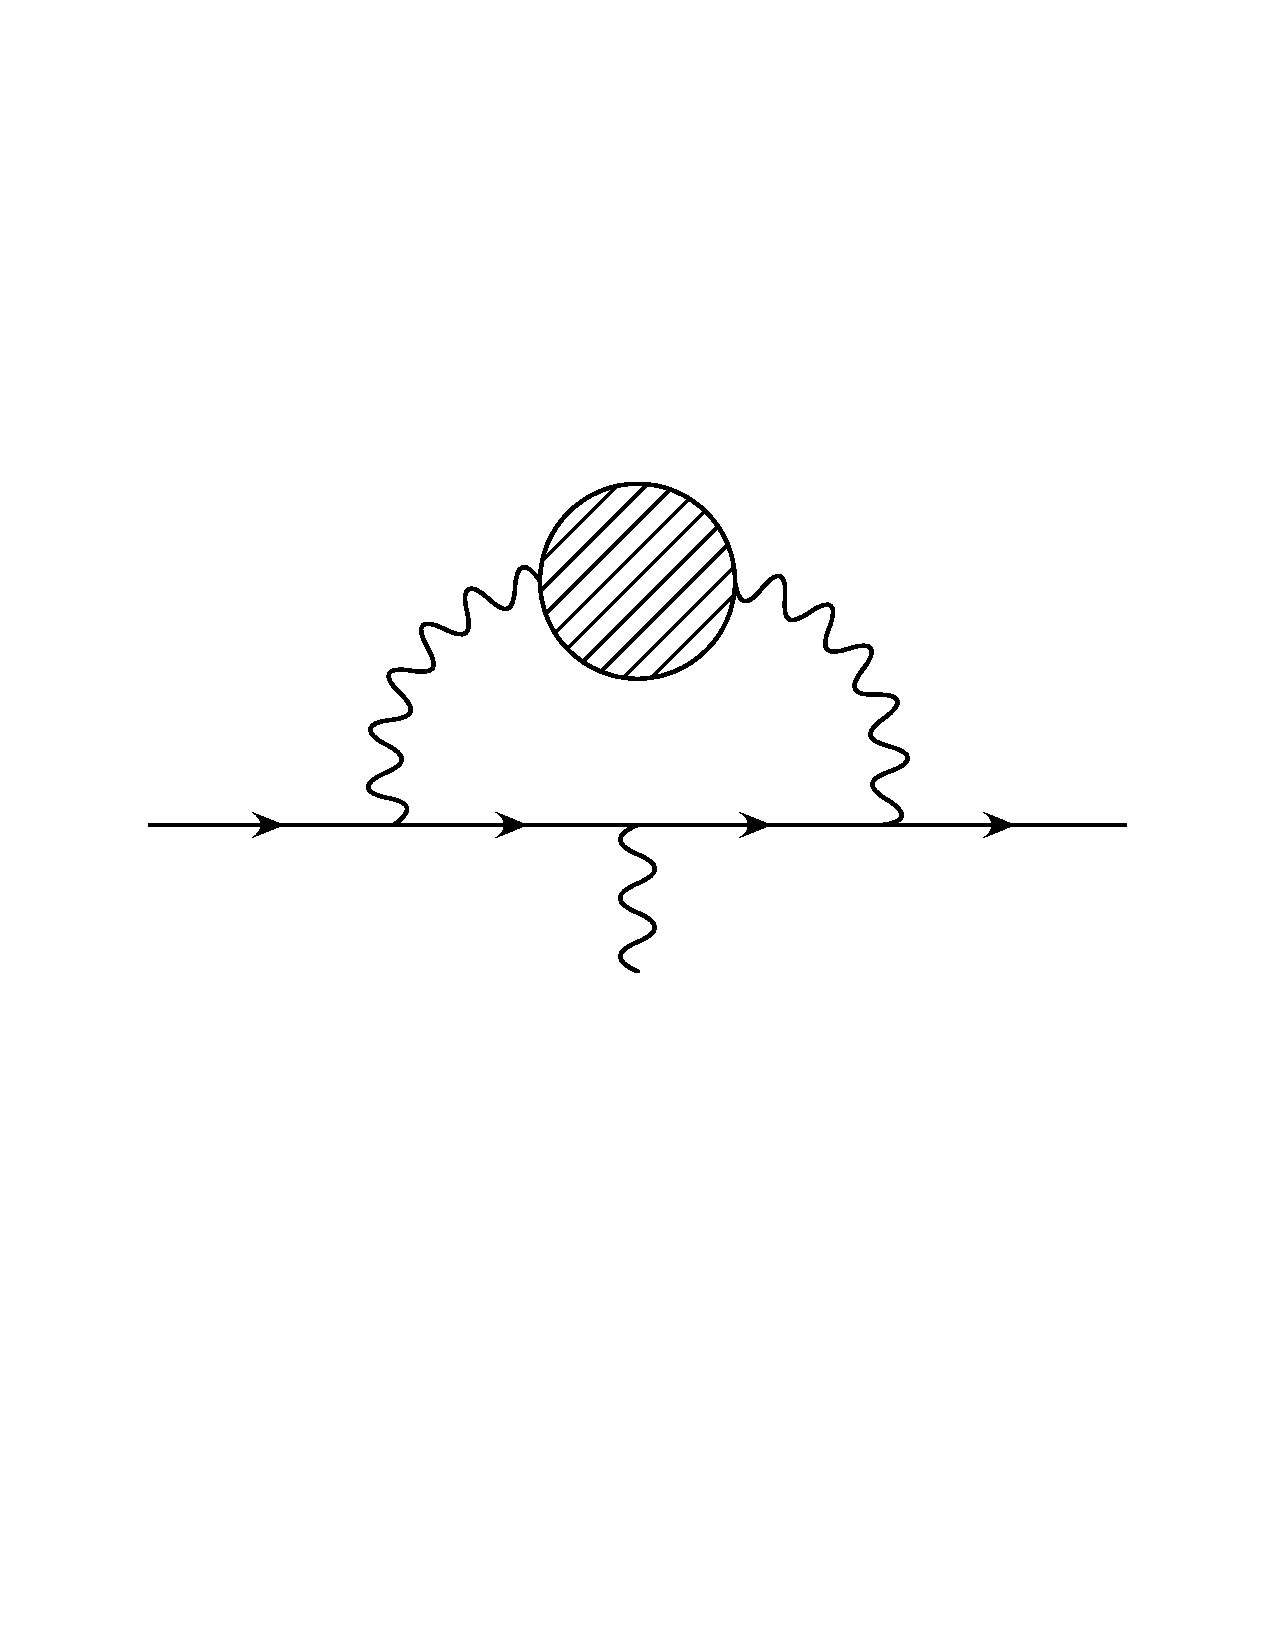
\includegraphics[width=0.3\columnwidth]{ChargedLeptons/Figures/hvp.pdf}\hskip 1cm
    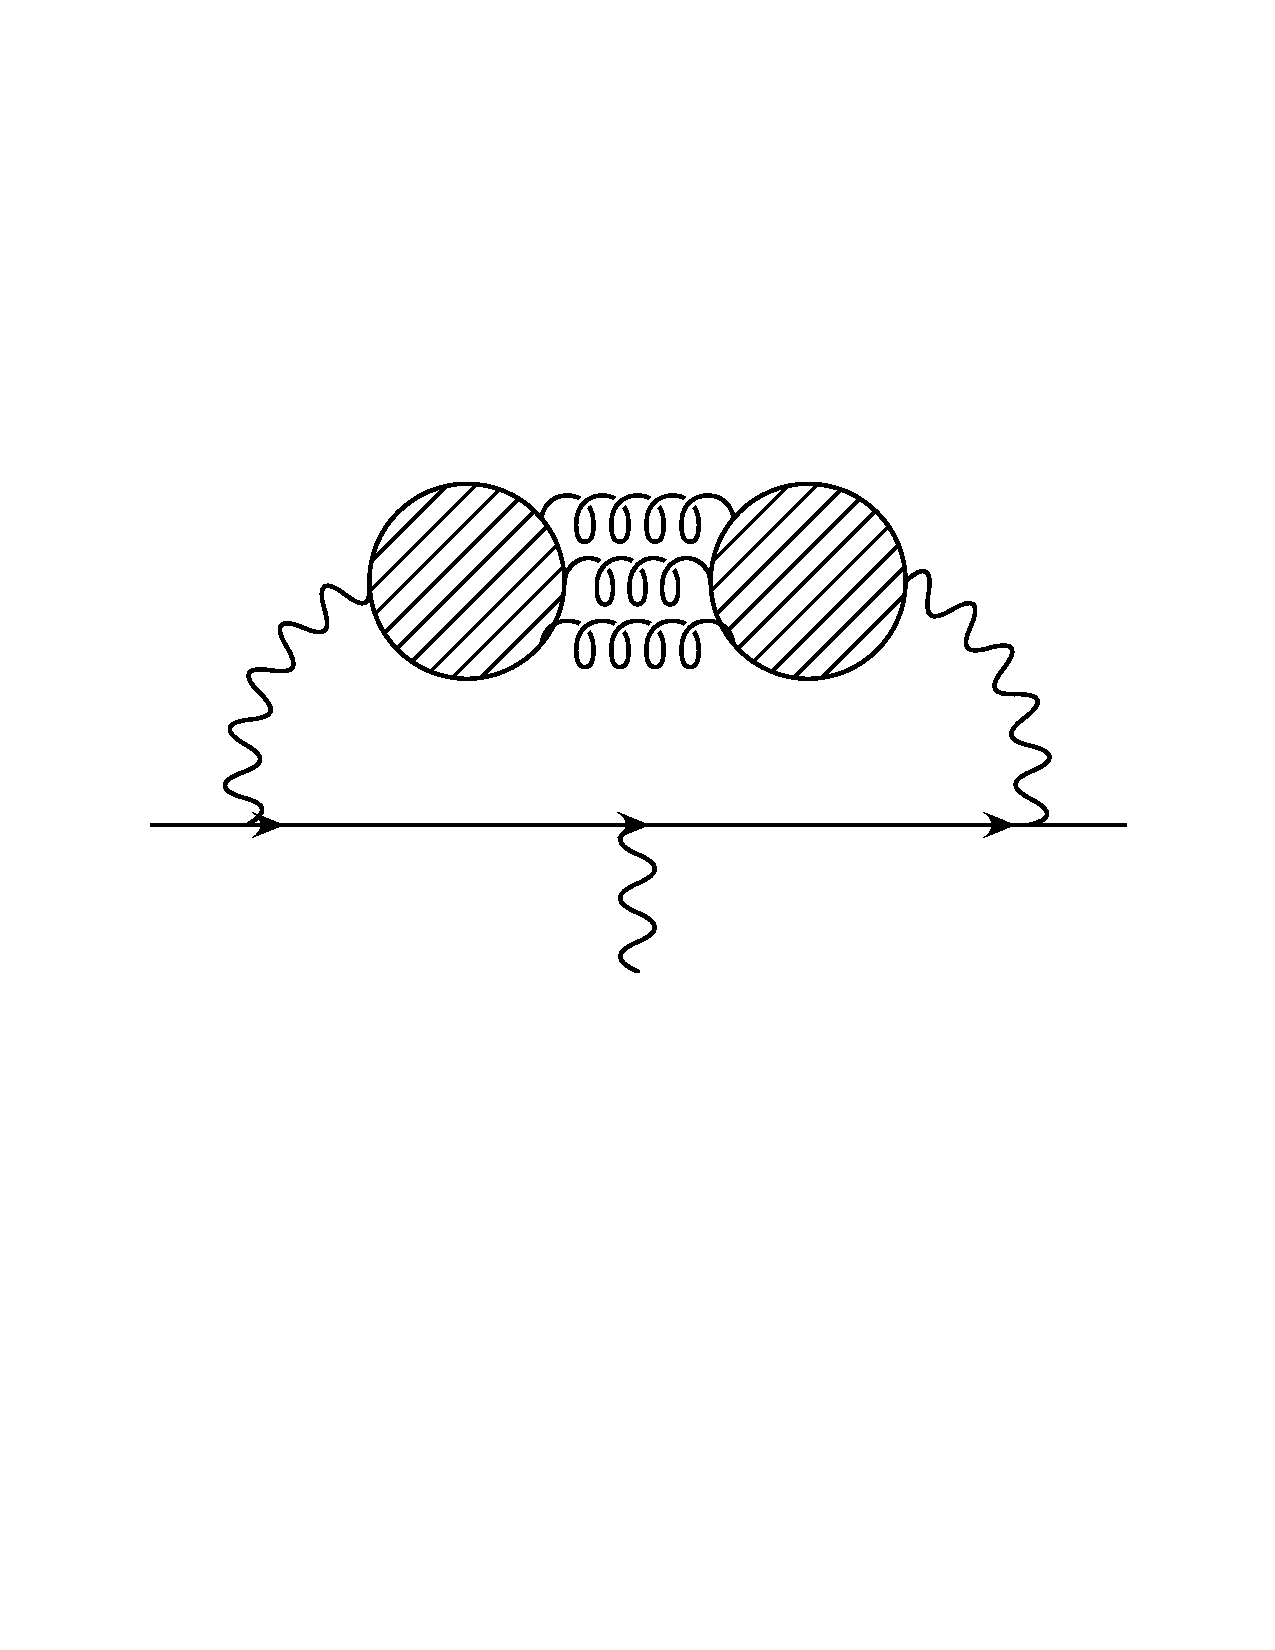
\includegraphics[width=0.3\columnwidth]{ChargedLeptons/Figures/hvp-disc.pdf}
\caption{Hadronic vacuum polarization diagrams contributing to the SM muon anomaly. The horizontal lines represent the muon. (Left panel) The blob formed by the quark-antiquark loop represents all possible hadronic intermediate states.  (Right panel) Disconnected quark line contribution. The quark loops are connected by gluons.}

    \label{fig:hvp}
\end{figure}
%

The hadronic-light-by-light (HLbL) scattering amplitude shown in
Fig.~\ref{fig:hlbl} is much more challenging.  The contribution to
$g-2$,
\begin{equation}
    a_\mu(\textrm{HLbL}) = 105(26) \times 10^{-11},
    \label{eq:PRV}
\end{equation}
is not well known. It is based on the size of various hadronic contributions estimated in
several different models~\cite{arXiv:0901.0306}.
Its uncertainty, though less than that in $a_\mu(\textrm{HVP})$ by about a factor of two, seems harder to reduce and is expected to be the dominant uncertainty as the HVP uncertainty is reduced.
Finding a new approach, such as lattice QCD, in which uncertainties are systematically improvable,
is crucial for making greatest use of the next round of experiments.
With this in mind, a workshop was recently convened at the Institute for Nuclear Theory~\cite{INTws}.
Workshop participants discussed how models, lattice QCD, and data-driven methods could be exploited to reduce the
uncertainty on $a_\mu(\textrm{HLbL})$.
The outcome of this workshop is that a SM calculation of the HLbL contribution with a total
uncertainty of 10\%, or less, can be achieved within five years. A detailed discussion of the computation of $a_\mu(\rm HLbL)$ in lattice QCD is given in the USQCD Collaboration white paper on $g-2$~\cite{USQCD}.
%
\begin{figure}[bp]
    \centering
\vspace*{-2pt}
    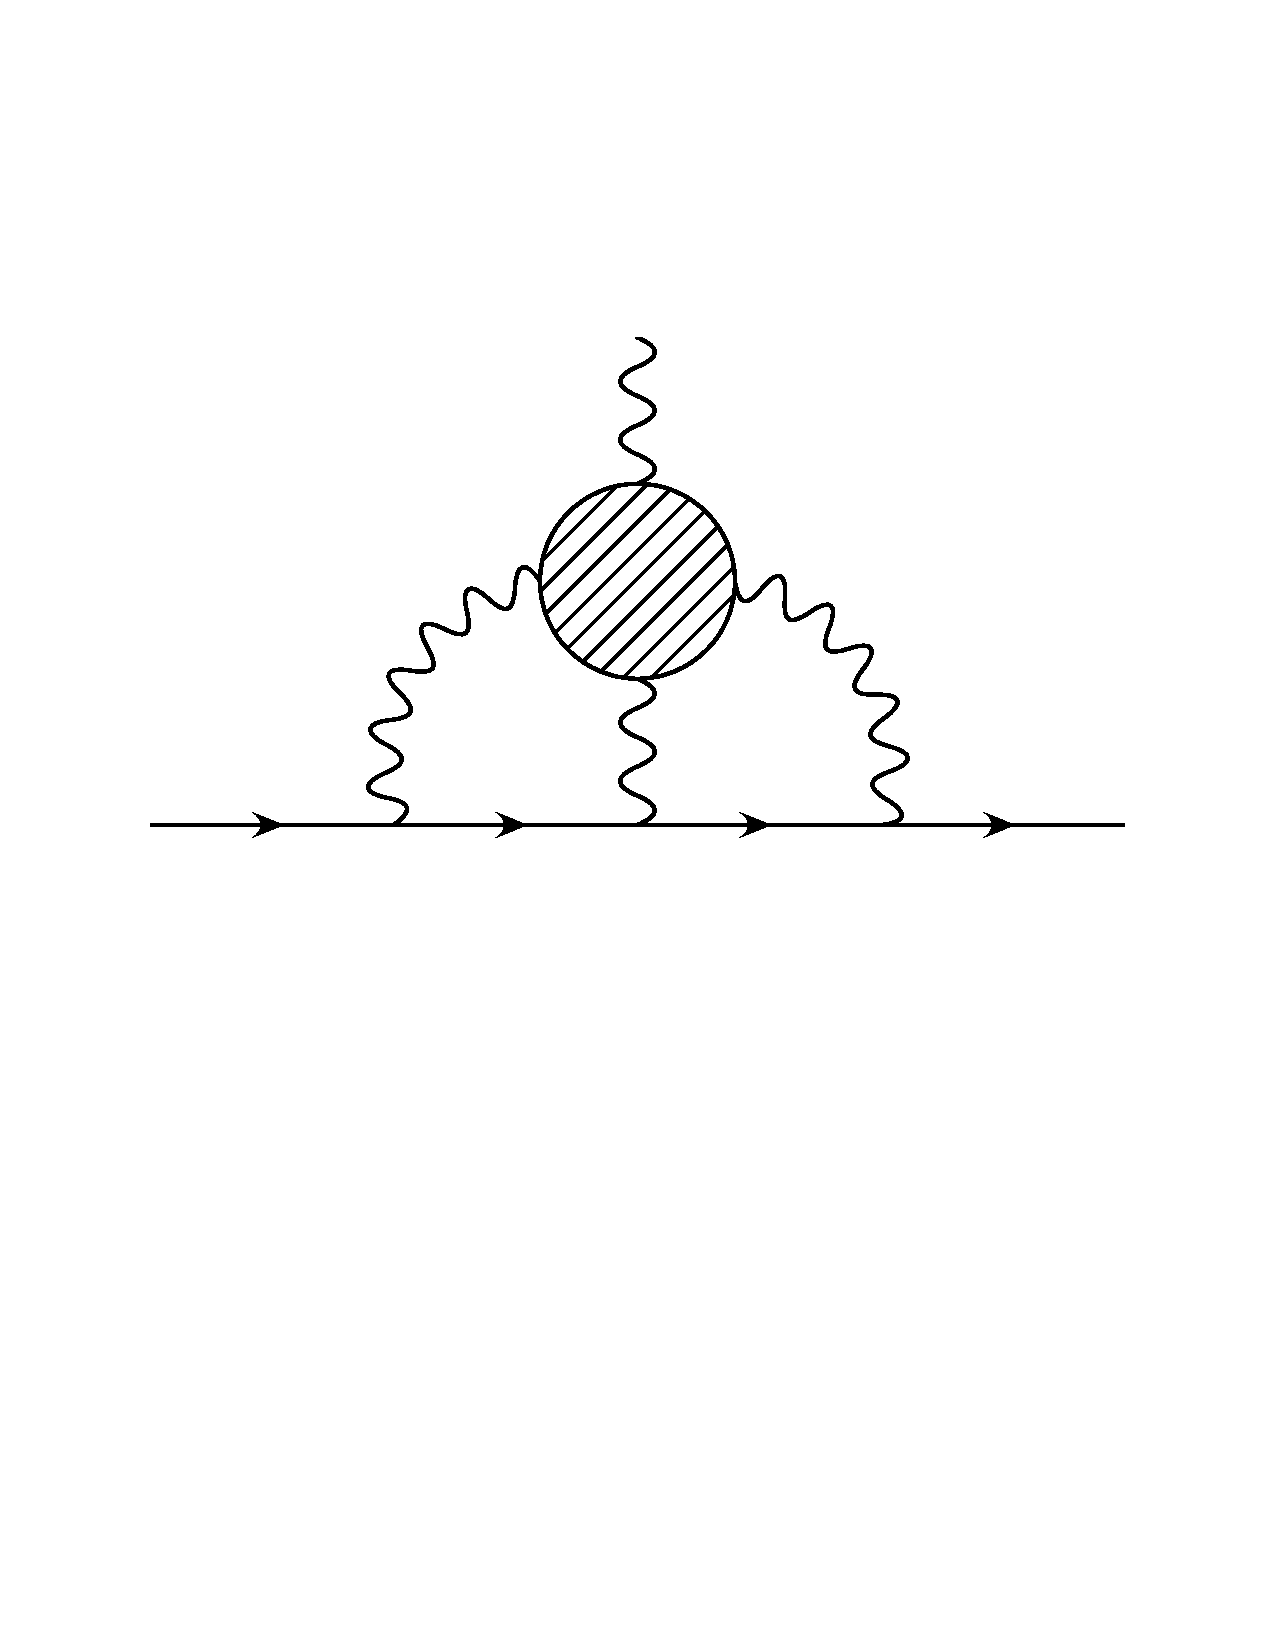
\includegraphics[width=0.3\columnwidth]{ChargedLeptons/Figures/hlbl.pdf}\hskip 1cm
    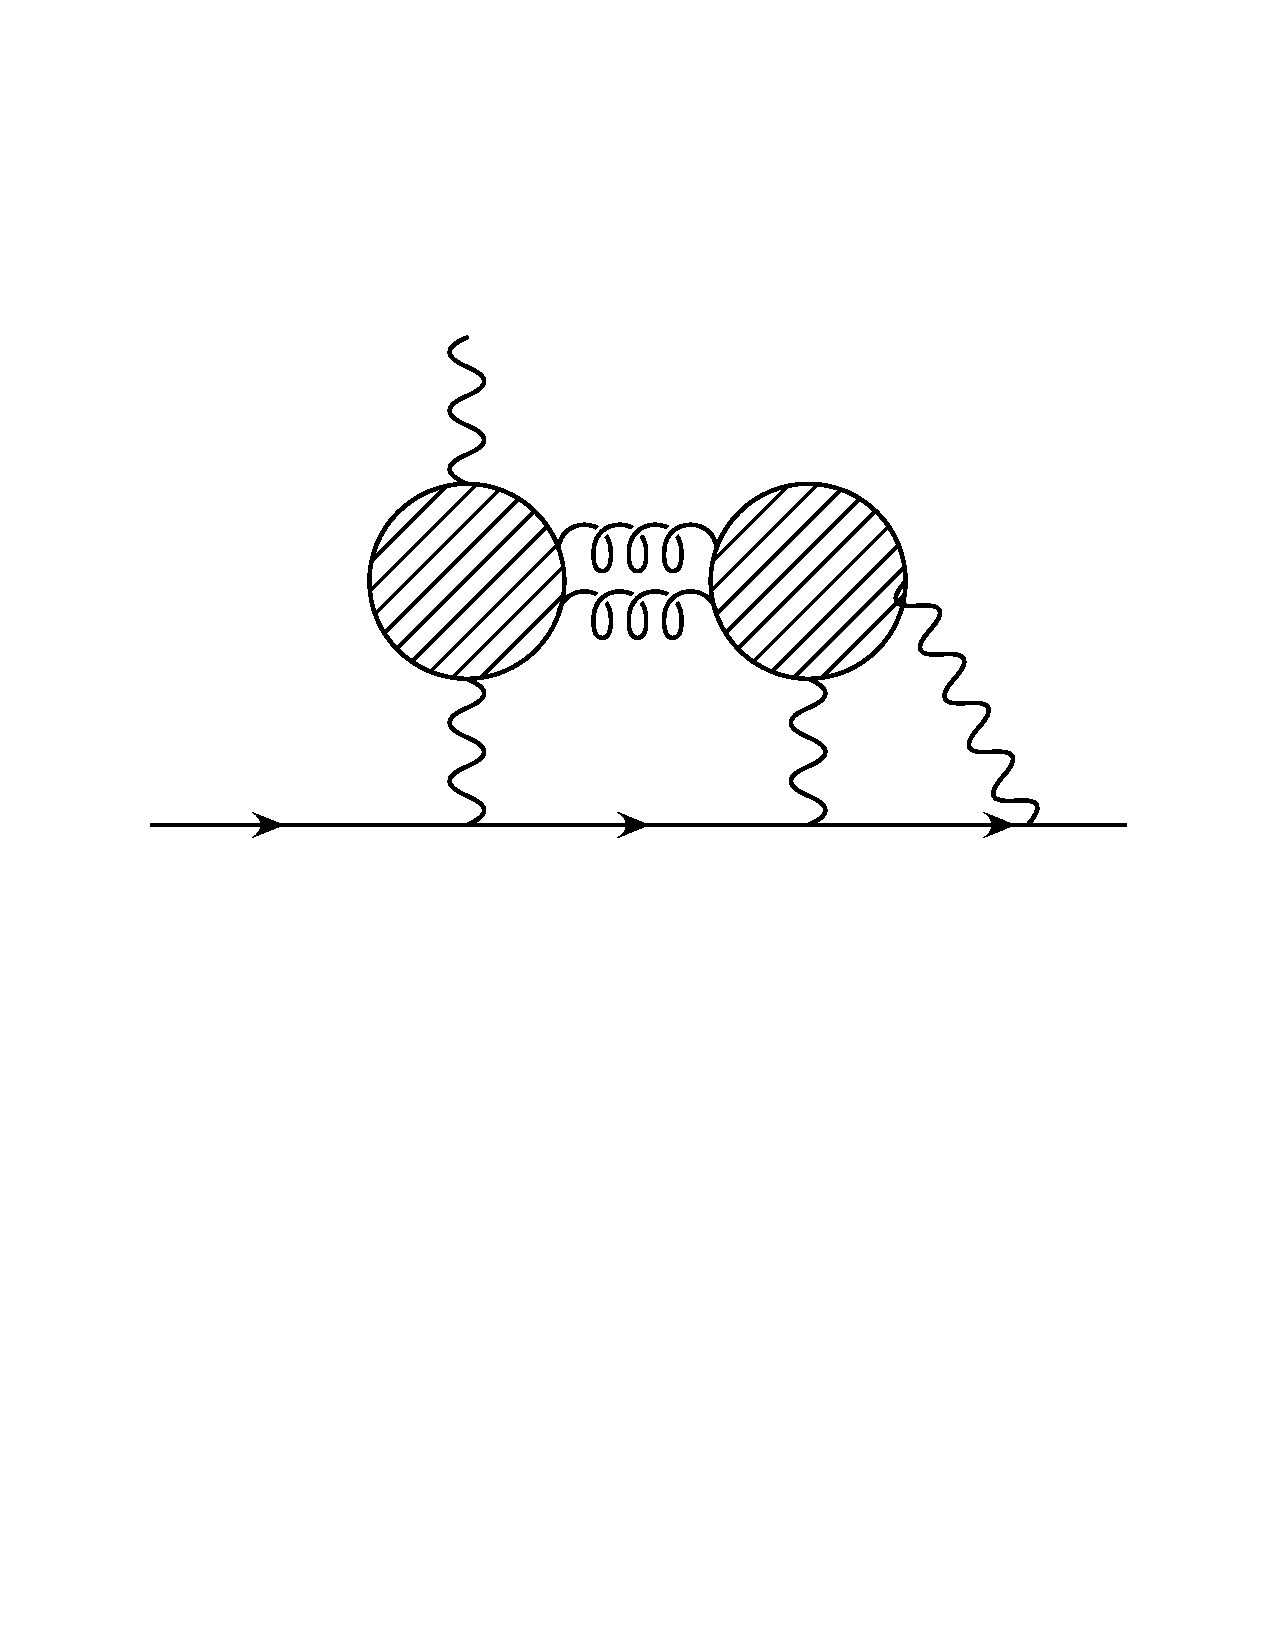
\includegraphics[width=0.3\columnwidth]{ChargedLeptons/Figures/hlbl-disc.pdf}
    \caption{Hadronic light-by-light scattering diagrams contributing to the SM muon anomaly. The horizontal lines represent the muon. (Left panel) The blob formed by the quark loop represents all possible hadronic intermediate states.  (Right panel) One of the disconnected quark line contributions. The quark loops are connected by gluons.}
    \label{fig:hlbl}
\end{figure}
%

There are two methods, using the lattice framework, under investigation. The conventional one, analogous to the HVP calculation, is to calculate the correlation function of four electromagnetic currents for the quarks in pure QCD, one for each possible, independent, momentum configuration (there are $V^2$), fit the resulting function of discrete momenta to a smooth function and insert it into the two-loop QED integrals. The resulting four-Lorentz-index hadronic tensor has 32 independent contractions. For these reasons, the calculation is computationally demanding. An intermediate but useful step is to calculate the four-point correlation function at well chosen values of the vertex momenta to partially check model calculations.

A second method is to compute the entire amplitude on the lattice, including the muon, in a  combined QED+QCD gauge field~\cite{hep-lat/9602005,hep-lat/0509016,827504}. The method has passed several non-trivial tests. First, it has been successfully checked against perturbation theory in pure QED. Large finite volume effects (the photons are long range) appear manageable. Preliminary calculations in full QED+QCD, at unphysical quark and muon mass and momentum transfer $q^2$, show a statistically significant result. The method requires a non-perturbative subtraction of leading order in $\alpha$ contributions which has been checked by varying the strength of the electric charge in the calculations and observing the expected scaling, before and after the subtraction. Disconnected contributions like the one shown in the right panel of Fig.~\ref{fig:hlbl} have not been included yet, but will be once the simpler first diagram (left panel, same figure) is fully under control. Calculations on a larger volume with smaller masses are in progress.

In addition to these direct approaches, there is other ongoing work on lattice-QCD calculations that check or
supplement the model calculations.
For example, it is well-known that the pion pole (namely, $\gamma\gamma^*\to\pi^0\to\gamma^*\gamma^*$)
provides the largest contribution to the QCD blob in Fig.~\ref{fig:hlbl}.
Just as experiments are being mounted to examine this physics (\emph{e.g.}, PrimEx at JLab and KLOE at LNF),
several groups~\cite{arXiv:0810.5550,arXiv:0912.0253,XFeng} are using lattice QCD to compute the amplitudes for
$\pi^0\to\gamma\gamma^*$ and $\pi^0\to\gamma^*\gamma^*$ (with one or two virtual photons).

If the SM and experiment central values do not change while both experiment and theory uncertainties are reduced, the discrepancy between the two becomes irresistible. The improvement expected from E989 (0.14 PPM) by itself improves $\Delta a_\mu$ to 5$\sigma$. A simultaneous decrease in the HLbL uncertainty to 10\% from the current 25\% pushes it to 6$\sigma$, and finally, reducing the uncertainty on the HVP contribution by a factor of two increases it to 9 $\sigma$. Such a large and clear difference between experiment and the Standard Model for the muon $g-2$ will be extremely  discriminating between new physics scenarios responsible for this discrepancy and will significantly leverage results from the energy frontier being explored at the LHC.



\subsection{Storage Ring EDM experiments}

At the magic momentum, the equation for the spin procession frequency of a charged particle in a storage ring is given by
\begin{equation}
\vec{\omega}_{a\eta}= \vec \omega_a + \vec \omega_\eta = -
 a \frac {Qe}  {m}
 \vec{B}
 -  \eta \frac {Qe}{2m}
 \left[ \frac {\vec{E}} {c}  +  \vec{\beta} \times \vec{B} \right] .
 \label{eq:omegaa-edm1}
\end{equation}
The precession frequency is by far dominated by the $a= (g-2)/2$ term.  
The key to extracting sensitivity to the EDM term $\eta$ is to find ways of reducing or eliminating the motion due to the magnetic term $a$. 

The first method is to use a magnetic storage ring such as the Muon g-2 experiment to extract a 
limit on the muon EDM.  In the muon rest frame, the muon sees a strong motional electric field
 pointing towards the center of the ring adding a small horizontal component to the precession 
 frequency vector that tilts the rotation plane.  For a positive EDM, when the spin is pointing into the 
 ring it will have a negative vertical component and when the spin is pointing to the outside of the ring 
 it will have a positive vertical component.  Since the positrons are emitted along the spin direction, 
 this asymmetry maps into the positron decay angle. Since the asymmetry is maximized when the spin 
 are perpendicular, the angular asymmetry is 90 degrees out of phase with the $g-2$ precession frequency.  
Searches for this asymmetry have been used to set limits on the muon EDM both at the CERN and Brookhaven $g-2$ experiments. 

 A number of the E989 detector stations will
be instrumented with straw chambers to measure the decay positron
tracks. With this instrumentation, a simultaneous EDM
measurement can be made during the $a_\mu$ data collection,
improving on the  E821 muon EDM~\cite{Bennett08-edm}
 limit by up to two orders of magnitude down to
$\sim 10^{-21}\,  e \cdot {\rm cm}$.   The J-PARC muon $g-2$ proposal also
 will have decay angle information for all tracks and expects a similar improvement.

To go beyond this level for the muon, will require a dedicated EDM experiment that
uses
the ``frozen spin'' method~\cite{Farley04,Roberts2010}.
 The idea is to operate a
muon storage ring off of the  $g-2$ momentum and to use a radial electric field
to cancel the $\omega_a$ term in Eq.~\ref{eq:omegaa-edm1},
 the $g-2$ precession.  The  electric field needed to freeze the spin is
$E \simeq aBc\beta\gamma^2$.
Once the spin is frozen, the EDM will cause a steadily increasing
out-of-plane motion of the spin vector. One stores polarized muons in a ring
with detectors above and below the storage region and forms the asymmetry
(up - down)/(up + down).  To reach a sensitivity of $10^{-24}e \cdot {\rm cm}$ would
require $\sim 4 \times 10^{16}$ recorded events~\cite{Farley04}.
 Preliminary discussions have begun on a frozen spin experiment
using the ~1000 kW beam power available at the Project X 3 GeV rare process campus.

An alternative method is to remove the $g-2$ precession frequency completely by removing 
the magnet and using an electrostatic storage ring. This still requires the particle to be at the 
magic momentum to cancel the motional magnetic field.  For these experiments, counter rotating 
beams are used to cancel the dominant systematic effects associated with stray magnetic fields.  
This idea has been studied in detail for the proton and deuteron with projected sensitivities approaching $10^{-30}$ 
using fairly large storage rings an proton momenta of $700$ MeV.

For the electron, the magic momentum is $15$ MeV.  The smaller momentum would allow for a
 much smaller storage ring.  Initial studies indicate that sensitivities up to $10^{-27}$ $\cdot $cm 
 can be achieved which would be competitive with current limits and would be the best limits for a
  bare fermion.  Furthermore, this would act as a much smaller test bed for the proton storage ring EDM experiment and would 
  help demonstrate that the systematic uncertainties could be controlled.
  
((((((((Add a few paragraphs about the details of the electron proposal))))))))


